\section{Implementation} \label{implementation}
In this project, both the VM emulator and the CPU emulator were implemented.
However, the decision to also implement the CPU emulator was made relatively late in the implementation process, as it was difficult to accurately estimate the time required to implement the VM.
The CPU emulator is also much simpler than the VM and can reuse some of the code from the VM implementation.
Accordingly, most of this section focuses only on the VM emulator.
If no emulator is explicitly specified, the text always refers to the VM.

\subsection{General approach}
With any project, one must first decide on a course of action.
Due to the relatively unique requirements of this project, the order in which the features are to be implemented is not immediately obvious.
There are basically two possible approaches.
A top-down approach would begin with the user interface (UI) implementation first and fill in the gaps later.
But since the application has different user interfaces depending on the intended use, it makes more sense to develop from the bottom up.
This allows for a more test-driven approach, where the internal logic of the emulator is developed first and only later integrated into the UI.
In order to be able to test the VM properly, it made sense to implement the bytecode parser first~\ref{parser-dev}, as it would significantly reduce the effort required to write unit tests for the VM.
Once the parser was completed, the VM could be implemented in isolation and independently of the future UI.
The various instructions of the VM vary in complexity, so it made sense to postpone the implementation of the Function, Call and Return instructions until all other instructions had been implemented and sufficiently tested.
Here the tests in the course projects, which were intended to test the participants' compiler implementation, helped to ensure the correct functionality of the emulator.
Although there was no way to parse the test scripts directly at this point, they were still very useful as they could easily be translated directly into Rust code by hand.
After all instructions were implemented according to their specification~\cite{nisan2005}, the emulator was fully functional and the standard library was simply loaded in its bytecode form, which made it possible to execute any VM program without modifications.
This approach unfortunately leads to performance issues, which is why the standard library was later reimplemented in Rust~\ref{jack-stdlib-in-rust}.

% \subsubsection{Test driven development of the VM without an UI}
% \begin{itemize}
%   \item first implement bytecode parser, because it can be used in VM Tests
%   \item basic VM features (everything except for function, call, return)
%   \item testing with unit tests (Translations of VME.tst tests)
%   \item rest of the VM instructions
%   \item stdlib only as vm bytecode
% \end{itemize}

\subsection{Architectural overview}
The general architecture of the application is outlined in \cref{fig:arch}.
Every box in this diagram represents a Rust module, which can either be a single file or an entire directory.
The architecture is divided into three major areas: the actual simulators, the parsers, and the interfaces that serve as entry points into the application.
Although the CPU and VM are commonly referred to as emulators, the module is called simulators because this is a more general term that also applies to the hardware simulator, which was not implemented as part of this work~\ref{future-work}.
This is the naming convention used by the official tools, where the emulators are also part of the simulators package~\cite{n2tsimulators}.
The two terms are therefore used interchangeably in the following sections.

\begin{center}
  \begin{figure}[ht]
    \centering
    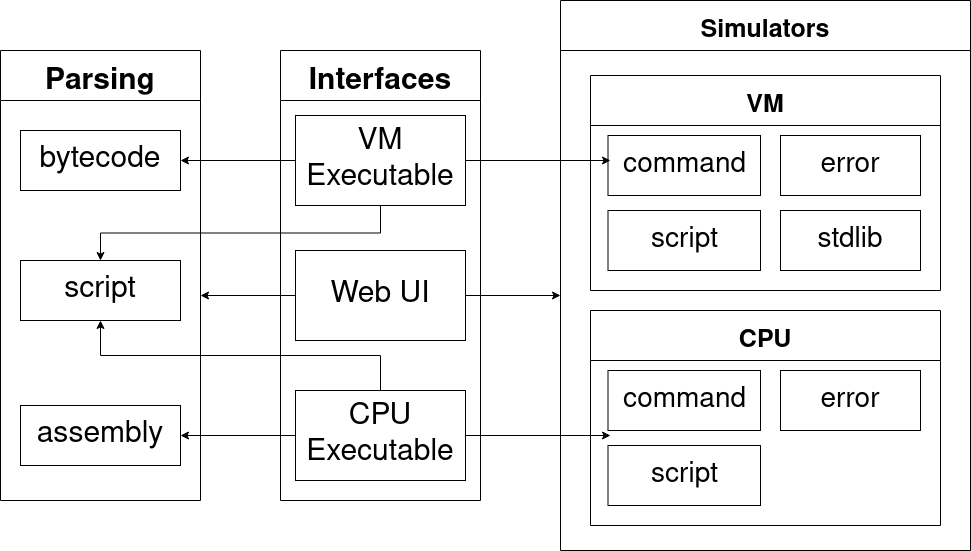
\includegraphics[width=12cm]{fig/architecture.png}
    \caption{Architecture overview diagram.}%
    \label{fig:arch}
  \end{figure}
\end{center}

\subsubsection{Interfaces} \label{interfaces}
There are three possible entry points for the application, listed in the ``Interfaces'' section of the figure.
Two of them are intended for use via the command line.
Both provide the ability to use the test scripts included in the project within the new emulator, but work in slightly different ways, as the VM emulator can run without a test script, while the CPU emulator does not currently have this capability.
For this reason, the VM emulator can either accept a path to such a test script or a path to a directory containing bytecode, while the CPU emulator accepts only a file path for a test script as input.
If the user passes a path to a directory, the application loads all files with the vm extension from that directory and then tries to execute them.
If a test script is passed instead, that script is executed as described in~\cref{test-script-workflow}.
In the first case, a window is displayed if the application was compiled with the desktop function enabled.
Otherwise, a message is printed telling the user that the application is running in headless mode.
Other options are also available to the user, such as the ability to set the tick speed or print the output of the test script to stdout instead of writing it into the output file described in the test script.
There is also the possibility to use the bytecode implementation of the whole standard library instead of the one written in Rust.
All of these options can be listed with the ``-h'' flag.

The third entry point is the most important for the majority of users.
The Web UI, a JavaScript application that calls the emulator implementations as a WebAssembly library, is easily accessible in any standard web browser.
Unlike the other two entry points, which can only use one of the emulators at a time, the Web UI can use both, indicated in the diagram by an arrow pointing to the outer simulator module.
Though test scripts are currently not supported here~\ref{future-work}.
This entry point can be used without the need to install additional software on the user's system by simply launching a web page in the browser.
The current address of this web page is given in the readme file in the root directory of the project.

\subsubsection{Simulators and Parsers}
The two emulators in the Simulators module are structurally very similar. Both have a Command module that contains the instruction enum~\ref{rust-vm-dev}, an Error module that contains the error enum for the respective emulator and a Script module that handles the emulators execution if run via a test script.
The VM is more complex, however, and also includes the Stdlib module, which contains the Rust implementation of the Jack standard library~\ref{jack-stdlib-in-rust}.

Unlike the simulators module, the Parsing module actually contains three different submodules, as the script parsing is mostly independent from the emulator implementation used.
All of the parsers share a lot of common code, so it makes sense to combine them into one module.
Having said that, there are some emulator specific instructions in the scripts, which were already highlighted in~\cref{test-scripts}.
The code to parse these special instructions is contained in the Script module of the respective emulator, instead of the module with the shared code.
This division was done intentionally, because parsing those instructions is only a small part of the whole script parsing process and is closely linked to the way the script is interpreted by the emulator.

\subsection{VM development in Rust} \label{rust-vm-dev}
The following section offer a mix of general techniques for VM development in Rust while explaining the specific choices made during the development of this project.
All processors and their emulators basically follow the same three-step cycle.
They first fetch the next instruction to be executed.
The internal number containing the current instruction is called program counter in the following sections.
After the instruction is fetched, it is decoded, i.e., the emulator determines what type of instruction it has just fetched and decodes the arguments for that instruction if necessary.
The final step is the actual execution, which is of course specific to the instruction in question~\cite{nystrom2021crafting}.

% \subsubsection{The internal representation of bytecode}
\label{bytecode-implementation}
Before starting to implement a VM, one must first decide on an internal representation for the bytecode that will run on that VM.
The design of the bytecode will always require a tradeoff between performance and ease of use during development.
In the original emulator implementation, a very inefficient representation was chosen where each instruction is an object of an instruction class.
This class contains a field for the opcode and several fields for possible arguments, as well as another integer that determines the number of arguments.
Using the example of \verb+push constant 3+, the opcode would be an integer that means \verb+push+, while \verb+constant+ and \verb+3+ would be the arguments, so the number of arguments would be two.
On top of that, it also contains a string argument that is used for call instructions, because functions are actually called by their name at runtime.
This design has several disadvantages from a performance standpoint.
Each instruction must be allocated on the heap and therefore requires pointer indirection during execution, which is known to have a drastic impact on performance as it reduces spatial locality~\cite{6498541}.
Furthermore, using strings to dispatch call instructions is a lot less efficient than just jumping to the correct bytecode position directly.

There are two basic ways to represent instructions in an emulator.
The choice between these two possibilities was a very important decision in the development of the new emulator.
Instructions can either have a fixed-size, or they can have variable-sizes.
Making all instructions the same fixed-size makes development simpler, as a single element in the program vector corresponds to a single instruction.
But representing an instruction set like the VM bytecode, where some instructions take arguments and others do not~\ref{table:vm-instructions} with a fixed-size, means that some instructions require padding.
\begin{center}
  \begin{figure}[ht]
    \centering
    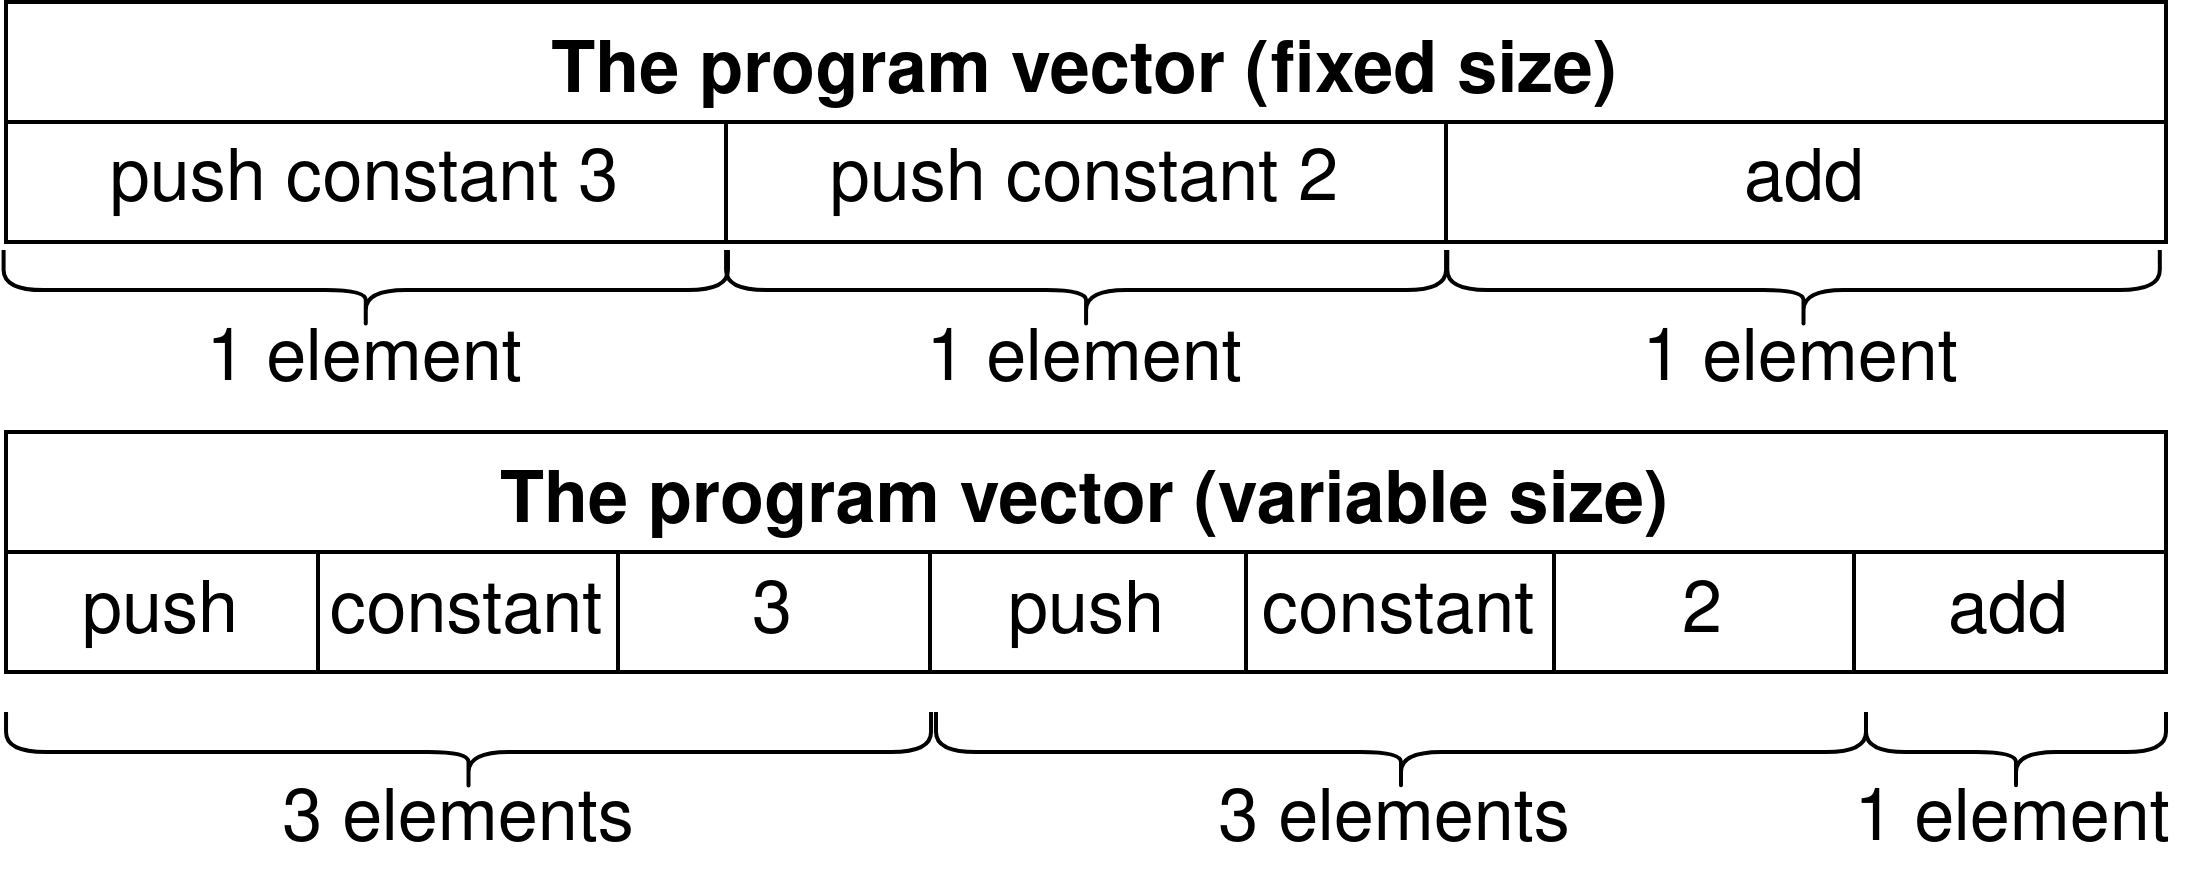
\includegraphics[width=12cm]{fig/instruction-size.png}
    \caption{The difference between fixed and variable-size instructions.}
    \label{fig:instruction-size}
  \end{figure}
\end{center}
In the fixed-size vector in~\cref{fig:instruction-size}, the add instruction has the same size as the push instructions.
Because the add instruction has no arguments and therefore stores less information than the push instructions, this wastes some space.
In constrast, the variable-size vector does not waste any space, but each instruction is now represented by multiple elements.
The instructions have essentially been split into bytes without any high level structure.
This leads to a significant issue.
A single instruction in the textual representation of the bytecode can now correspond to multiple entries in the instruction vector, e.g.\ \verb+push constant 3+ requires three entries in the program vector.
As a result, the index of an instruction in the program at runtime is often significantly larger than the line number of the same instruction in the input.
% The first and less important is that additional metadata is required to determine the line number in the input from the current instruction in the runtime representation, which drastically increases the complexity needed to implement the code view in the UI.
This is a problem because jump instructions in hack bytecode are absolute, i.e., a jump must know the index of its target instruction in the program vector, not just the position relative to itself.
By assigning multiple indices to each instruction, the index of each element in the vector becomes larger.
For example, the add instruction in the fixed-size representation in~\cref{fig:instruction-size} has the index two, but in the variable-size vector its index is actually six.
Since the number of possible indices is limited, this leads to a significant reduction in the amount of available jump locations, which makes it impossible to load larger projects like Hackenstein~\ref{fig:hackenstein-official}.
% Alternatively, we could dispense with the one-to-one mapping of addresses and bytecode indices, but that would further complicate the VM implementation.
A similar problem has already been discussed in~\cref{pynand} to explain why translating bytecode to assembly is not a good solution for this project.

For these reasons, the new emulator uses the fixed-size bytecode representation instead, similar to the official emulator but with some improvements.
It is not implemented with heap-allocated objects, but with enums~\ref{lst:enum-bytecode}.
These allow the programmer to define a type by enumerating its possible variants~\cite[Chapter~6]{klabnik2019rust}.
In the official emulator, the program vector only contains pointers to instruction objects on the heap, but enums can be stored directly in the vector, without any indirection.
On top of that, call instructions in the new emulator are not dispatched based on the function name.
Instead, the bytecode parser already resolves the name to the function's index within the bytecode vector~\ref{bytecode-parser}, so the VM can simply set the program counter directly to that value.
\begin{lstlisting}[
  language=Rust,
  label={lst:enum-bytecode},
  caption={The bytecode representation used in the final implementation.},
  captionpos=b
  ]
  pub enum Instruction {
    Add,
    Sub,
    // [...]
    Push { segment: Segment, index: Word },
    Pop { segment: Segment, index: Word },
    Function { n_locals: Word },
    Call { function: Word, n_args: Word },
  }
\end{lstlisting}
The size of an enum depends on the size of its largest variant, so padding bytes must be added at the end of smaller variants.
In this case, how can the disadvantage of wasting space in smaller instructions be justified from a performance standpoint?
To understand the impact of such design decisions, it is important to keep in mind the composition of actual bytecode programs.
By writing a small program that groups the lines of all bytecode files in a directory based on their first word, one can analyze the frequency of different instructions in VM programs.
Analysis of several different Jack programs~\ref{table:tested} and the Jack standard library showed that push and pop together account for about 70\% of all bytecode instructions in real programs, while call instructions make up another 10\%.
Not storing the function name in a call instruction has the additional benefit of making the Call instruction, which would otherwise be the largest variant, the same size as the push and pop instructions~\ref{lst:enum-bytecode}.
Since these instructions have the same maximum size and make up 80\% of all instructions, only 20\% of instructions need padding at all.
Based on this, the padding caused by using enums is not really relevant for the memory requirements and cache efficiency of actual programs.
Compared to the bytecode representation in the official emulator, this enum based approach is also still more efficient because it contains no pointers and therefore no indirections.
The enums are stored directly inside the vector, not in separate heap allocations.
Not resolving functions by name at runtime should also improve performance significantly.

Enums are typically used in conjunction with pattern matching, a feature that allows the programmer to compare a value against a series of patterns and then execute code based on which pattern matches~\cite[Chapter~6.2]{klabnik2019rust}.
This makes it very easy to not only identify the current instruction, but also extract all the necessary data from it.
With this approach, an entire instruction with all of its arguments is now contained in a single instance of the instruction enum.
\cref{lst:bytecode-pattern-matching} shows how pattern matching can be used in combination with enums to implement the decoding phase of the VM cycle in a clear and concise way by directly extracting the arguments of, for example, push and function instructions and binding them to new local names.
For the above reasons, the fixed-size enum-based representation is a good choice, both for performance and usability during development.
The exclamation mark in \verb+tos_binary!+ marks this expression as a call to a macro rather than a function, so the operator \verb*=+= can be passed as an argument.
\begin{lstlisting}[
  language=Rust,
  label={lst:bytecode-pattern-matching},
  caption={Using pattern matching to deconstruct the instruction data.},
  captionpos=b
  ]
  match instruction {
    Add => tos_binary!(self, +),
    // [...]
    Push { segment, index } => {
      let value = self.get_value(segment, index)?;
      self.push(value)?;
    }
    // [...]
    Function { n_locals } => {
      // initialize all local variables to zero
      for _ in 0..n_locals {
        self.push(0)?;
      }
    }
  }
\end{lstlisting}

% \subsubsection{Step by step execution with pattern matching}
\label{step-by-step}
The architecture with its different entry points and ways to use the emulators~\ref{fig:arch} places unique demands on the VM implementation.
In order to satisfy all those requirements, the VM runs in a way that executes one step at a time and is able to be suspended after each of those steps.
This constraint will be especially important for the interaction with native rust code in the standard library~\ref{jack-stdlib-in-rust}.
In each step, the VM first fetches the current instruction from the loaded program, then performs pattern matching to extract all the required data and finally executes the instruction.
The matching process can be seen in \cref{lst:bytecode-pattern-matching}, where the segment and index of a push instruction are extracted and then used to first load the value with another method and then push it onto the stack.
Rust's pattern matching handles the selection of the correct branch automatically.

\subsection{Parser development in Rust} \label{parser-dev}
Parsing usually consists of at least two stages, the first being lexical analysis, also known as tokenization.
At this stage, the individual characters of the input are grouped into tokens, which are assigned tags such as symbol, number, or keyword.
This is followed by the actual parsing stage, where the tokens are further grouped into constructs, such as arithmetic expressions or loops.
In its simplest form, a token is a tuple of a piece of the original source code, called a lexeme, and the tag that assigns a specific meaning to the lexeme.
% Some things, such as parsing integer literals from strings into actual numbers, can be done either within the lexer or, alternatively, only during the actual code generation or interpretation of the program~\cite{nystrom2021crafting}.
Neither assembly~\ref{hack-assembly} nor bytecode~\ref{hack-bytecode} really have any complex constructs, since both are already flat lists of instructions.
The test scripts~\ref{test-scripts}, on the other hand, also contain more complex instructions, such as repeat, which is essentially a for loop.

\subsubsection{Generic lexer}
Much of the lexical analysis code can be shared by all three parsers.
At its core, a lexer only needs to consume characters as long as certain conditions are met, and then return a token containing those characters, their position in the original source code for error reporting, and the type of token that was consumed.
Taking characters based on a condition and then combining them with location information is independent of the particular parser.
This is why this functionality is implemented in a generic lexer, which is used by all three parsers.
The generic lexer offers a method \verb+take_chars_while+, which again takes a higher order predicate function as its argument.
This predicate function is evaluated for each character, starting from the current position of the lexer, until it returns false for the first time.
Then all characters that evaluated true when applied to the predicate are returned as a single string with information about the strings's position in the entire source code.
A possible predicate might be \verb+char::is_numeric+ which tests if a given character is a digit.
So calling \verb+generic_lexer.take_chars_while(char::is_numeric)+ would consume an entire number from the input string and return it wrapped in a span.
\label{spans}
The span is a structure that can wrap any generic inner type with information about its position in the source code, e.g.\ the line where the element occured.
This information can later be used to improve error messages for the programmer by indicating not only what went wrong, but also where the error happened.

% \subsubsection{Peekable as an example for the usefulness of traits}
% Each parser has its own lexer, which in turn uses the generic lexer internally.
% The lexers themselves are quite simple.
% They simply encode the rules for each token into predicates, which are then passed to the generic lexer, and then convert the string returned by that lexer into the correct token type.
% To provide a more uniform interface, these lexers also implement one of Rust's most important traits, the Iterator trait.
% This interface allows the use of types within for-each loops by providing a ``next'' method that can return the next element or nothing.
% This would be useful in and of itself, but Rusts powerful type system offers the ability to extend types that satisfy certain conditions by wrapping them with other types that offer even more functionality.
% One such type is called Peekable, which can be wrapped around any other type that implements the Iterator trait, allowing the user to peek at the next item without actually consuming it.
% Rust calls features like this ``zero cost abstractions'' because there is no runtime overhead compared to adding the functionality directly to each lexer.
% It is not implemented via dynamic dispatch, but is fully resolved at compile time.
% In addition, the Peekable type itself also implements the Iterator trait, so it just extends the interface without removing any functionality.
% Any type that implements the Iterator trait automatically has a ``peekable'' method that returns the Iterator instance wrapped in this type.

\subsubsection{The bytecode parser} \label{bytecode-parser}
The bytecode parser is the simplest of the three parsers.
As shown in~\cref{lst:hack-bytecode}, it is a flat and simple format, with simple and well-defined rules.
Nevertheless, it has some complexity due to the way symbols are resolved.
Functions and labels both declare symbols, which can be referenced before they are declared.
This is relevant because, as described in~\cref{bytecode-implementation}, call instructions and labels are resolved into indices in the program vector during parsing.
To achieve this, the parsing is divided into two different steps.
The first step is to parse the source code from beginning to end.
At this stage, the bytecode vector does not yet contain the completed instructions.
It instead contains instances of an enum, which can either be a fully resolved instruction or a partially constructed instruction with a symbol it is waiting for.
While reading the source code, the parser keeps track of all declared functions and labels.
When such an symbol is referenced in the code, the parser tries to find it in the environment.
If the symbol is already declared, the instruction is inserted into the result vector as a fully resolved instruction.
However, if the instruction references an undeclared symbol, the instruction is inserted with a placeholder and another string with the name of the missing symbol.
These placeholders are then replaced with the correct indices in the second stage.
Here the parser iterates over the previous result vector and handles any instructions with placeholders.
\begin{center}
  \begin{figure}[ht]
    \centering
    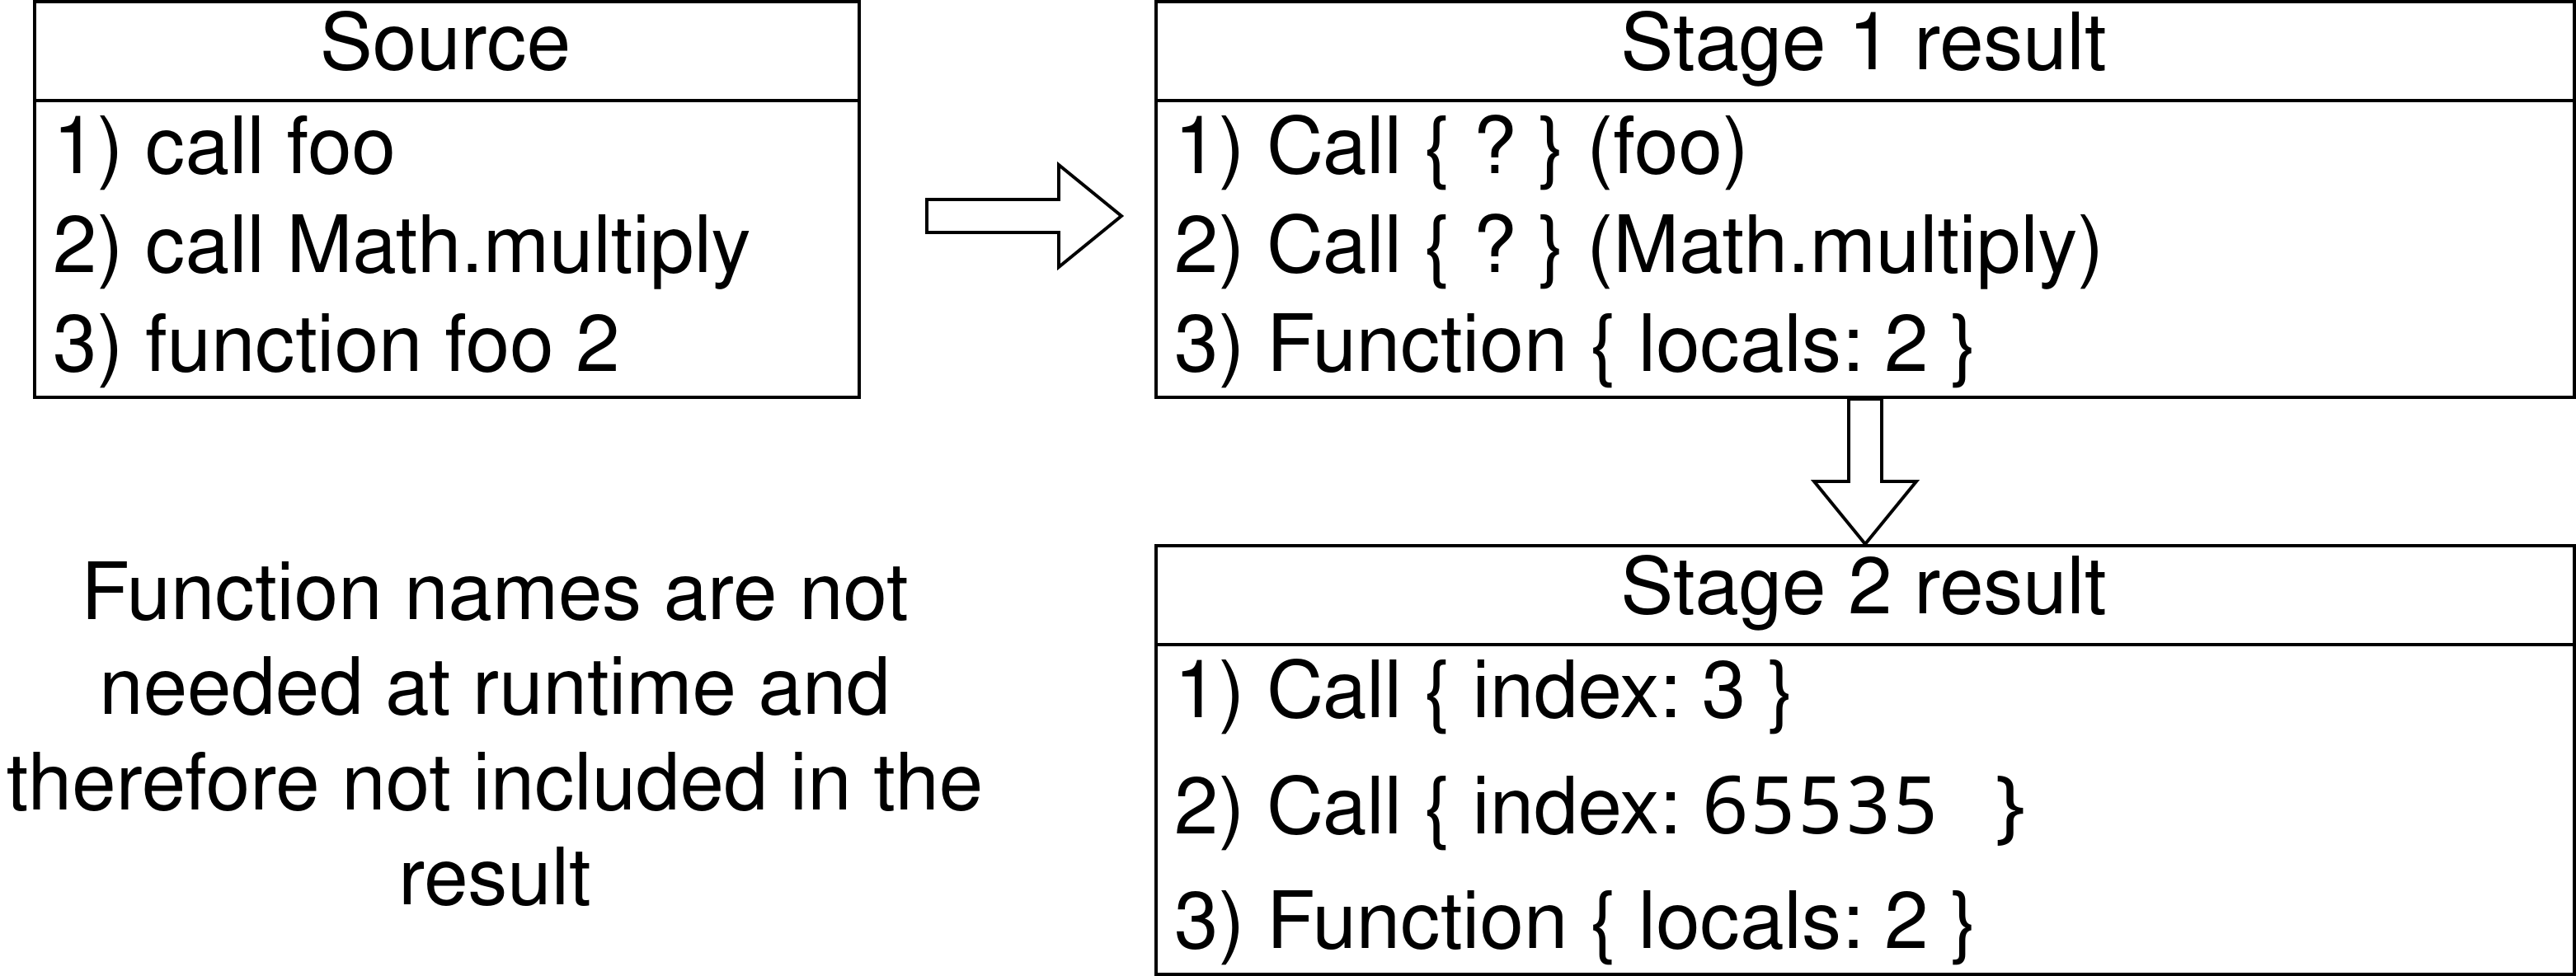
\includegraphics[width=12cm]{fig/bytecode-parsing.png}
    \caption{The two stages of bytecode parsing.}
    \label{fig:bytecode-parsing}
  \end{figure}
\end{center}
At the end, the parser performs a final check to see if there are any unresolved symbols left.
Should this be the case, it returns an error, otherwise the parser is done.
One thing which has yet to be explained: If function dispatching is based on the function's index in the program's bytecode vector, how are built-in standard library functions called?
These functions are not part of the bytecode and therefore not included in the parsed program.
They are assigned the highest possible addresses that would be valid indices into the bytecode vector.
So if \(N\) is the largest integer that still fits into the index type, and if \(n\) is the number of standard library functions, then the addresses in the range \([N - n + 1, N]\) are used to call those functions.
These addresses are not really part of the bytecode, they are just numbers known to the emulator that resolve to the implementation of a function in the native standard library, rather than a real bytecode instruction.
The exact index for each standard library function is determined before parsing, so the parser can simply replace any symbol referring to such a function with the correct index.
The connection between this index and the associated symbol can be resolved bidirectionally, so the VM can also resolve any call with an index greater than \(N - n\) to the appropriate native function.
The entire process can be seen in~\cref{fig:bytecode-parsing}, were the \verb+foo+ call is resolved to an actual index in the result, while the \verb+Math.multiply+ call is resolved to the highest possible index.

\subsection{The test script workflow} \label{test-script-workflow}
To allow automatic testing of student submissions, the Nand to Tetris course includes test scripts for most of its projects.
% These scripts are able to load programs depending on the emulator, set internal values in the emulator's memory, execute the program in a certain way, and then compare the values at specific memory addresses in the emulator with expected values loaded from a file.
% This functionality is not only useful for students, but also for the instructors of the course.
As described in~\cref{test-scripts}, these scripts share most of their functionality and syntax between all three simulators, but there are some simulator-specific features that pose a challenge to implementation.
The application must know which emulator the script is to be run in, so that only the correct instructions are parsed and executed.
Since the different emulators actually produce different executables~\ref{interfaces}, the emulator is already known, but it is not immediately obvious how to structure the code to allow only some of the possible commands to occur and be executed based on the current interface, while sharing as much code as possible.

% \subsubsection{Traits as an alternative to inheritance}
In an object-oriented language, functionality like that described above would probably be implemented using abstract classes or interfaces.
There might be an abstract test script parser from which the specific parsers for the VM, CPU, and hardware simulator would inherit.
The simulators could also inherit from an abstract script executor class that would implement most of the commands, leaving only the emulator-specific commands to the subclasses.
While Rust supports dynamic dispatch, it does not provide inheritance as a feature of the language.
But it does offer a powerful system of type parameters and traits to specify constraints on those types.
Methods can be implemented not only directly on types, but also conditionally if a combination of types matches certain properties.
The generic test script parser expects an emulator-specific command parser as its type parameter.
All methods of the generic parser are not actually implemented directly on this parser.
They are instead only implemented if the combination of the generic base parser and the simulator-specific parser together implement the ScriptParser trait.
The actual implementation of the parser interface is therefore not part of the module containing the generic parser.
Rather, it is implemented in the simulator-specific modules.
This process is more complicated than the object-oriented solution, but has the advantage of working without dynamic dispatch.
The type parameters for the simulator-specific commands can also be used to guarantee that the emulator really expects the same commands that the parser returns.
The code is presented in a simplified version in~\cref{lst:generic-parser} and~\cref{lst:vm-parser}.
In the real program, this code is more complicated due to some details of the Rust type system that do not add to the understanding of the core principles at work, so those have been omitted.

\begin{lstlisting}[
  language=Rust,
  label={lst:generic-parser},
  caption={The generic base parser for test scripts},
  captionpos=b
  ]
  // P is the simulator specific parser
  // C is the simulator specific command
  pub struct ScriptParser<P, C> {
    // fields like the peekable lexer
    [...]
  }

  impl ScriptParser<P, C>
  where ScriptParser<P, C>: SimulatorCommandParser<C>,
  {
    [...]
  }
\end{lstlisting}

The ScriptParser implementation block only becomes relevant if there is an emulator-specific parser that implements the missing parts, as shown for the VM emulator parser in~\cref{lst:vm-parser}.
Here the SimulatorCommandParser trait is implemented for the ScriptParser in combination with the specific VMEmulatorCommandParser, neither of which would implement the trait on their own.
This implementation has to contain the missing parse function for VM specific commands.

\begin{lstlisting}[
  language=Rust,
  label={lst:vm-parser},
  caption={The VM emulator specific parser for test scripts},
  captionpos=b
  ]
  pub struct VMEmulatorCommandParser {}

  impl SimulatorCommandParser<VMEmulatorCommand>
  for ScriptParser<VMEmulatorCommandParser, VMEmulatorCommand>
  {
    [...]
  }
\end{lstlisting}

% \subsubsection{Compile time check for the combination of parser and executor}
So far we have looked at the implementation of the test script parser, but of course the scripts need to be executed to be useful.
Just like parsing, most of the logic is shared among all simulators, which means that individual emulators should implement only the commands that are unique to them and share all other code.
The trait that specifies these methods also has a generic type parameter, just like the ``C'' parameter in~\cref{lst:generic-parser}.
This ensures at compile time that the parser and executor are compatible.
Rust's powerful type inference even allows it to determine the correct script parser implementation based on the executor provided.
The various interfaces can simply call the \verb+execute_script+ function with one of the simulators as its argument and the compiler will automatically infer the correct parser.

\subsection{The native standard library protocol} \label{jack-stdlib-in-rust}
Theoretically, the VM could simply use the implementation of the standard library written directly in bytecode.
From a functionality point of view, this implementation is almost identical to the Java implementation in the official emulator~\ref{sys.wait-example}.
The reason the official emulator still has a version of this library implemented in Java is the same reason the new emulator has a Rust version of the standard library:
It is much faster.
A simple example to show the huge impact is \verb+Math.multiply+.
The VM does not have its own multiply instruction, but relies on a software solution within the standard library.
During code generation, the compiler automatically converts any multiplication in the source code into a call to this function.
The multiplication function contains 92 lines of code with calls to \verb+Math.abs+ and a loop that executes 16 times, once for each bit in the two-byte integer.
A simple multiplication therefore requires hundreds of VM ticks to execute.
In the native Rust implementation, it requires only a single tick.
Other, more complicated functions may be executed less frequently, but the performance impact here is even greater.
Providing a native implementation of these functions is therefore one of the most important possible performance improvements.
Unfortunately, it is not trivial to provide such an implementation for several reasons.

\subsubsection{The issues with native functions in the virtual machine} \label{stdlib-issues}
There are several problems with integrating native code with bytecode.
First and foremost is the fundamentally different execution model.
The VM runs tick-based, i.e.\ it executes one instruction per tick, so it is possible to stop after each instruction.
This is not the case with Rust code, as we cannot stop a function in the middle of execution and resume it at a later time.
It is also not possible to simply run the entire function to completion within a single VM tick.
Some functions in the standard library run in an infinite loop, such as \verb+Keyboard.readLine+, which does not return until the user presses the Enter key on their keyboard.
Another difficult function is \verb+Sys.wait+, which takes a number as input and waits approximately that many milliseconds.
Targeting the web browser makes this function difficult to implement, as WebAssembly does not support multiple threads at the time of writing.
\verb+Sys.wait+ cannot block the only available thread, because this would cause the entire application to become unreponsive.
The implementation is further complicated by the fact that the communication is bidirectional.
Jack's standard library may only be partially implemented natively and partially as VM bytecode.
This is especially likely in Project 12, where students are expected to implement the standard library themselves.
Some functions of the standard library depend on other functions of the standard library, such as \verb+Output.printString+, which must call \verb+String.length+ to work.
The call to the actual length function is important here because the internal representation of strings is not part of the specification, only the interface.
To summarize, the bytecode must be able to call native Rust functions, and these native Rust functions must in turn be able to call functions implemented in bytecode.
In addition, there must be a way to stop the native functions like any other bytecode function, with the ability to resume execution at any time in the future, either based on user input, elapsed time, or other conditions.
The official implementation can work around many of these problems by using multiple threads that can actually be paused and resumed based on conditions.
Since this is not possible in WebAssembly, a new way of handling native standard library functions is required.

% \begin{itemize}
%   \item step by step execution -> no waiting
%   \item vm functions can call rust functions
%   \item rust functions can call vm functions
% \end{itemize}

\subsubsection{Solving those issues with a Finite-state machine}
To solve the problems described above, the new emulator uses finite-state machines.
Finite-state machines (FSMs) are a common model in computer science with a wide range of applications.
An FSM can only ever be in one of a finite number of states and can transition between these states based on conditions~\cite{sakarovitch2009elements}.
The functions in the Jack standard library do not need to be able to pause at any point in the code.
Instead, there are certain points at which the function can be paused, such as by calling another function, whether a VM or a native function, or by explicitly waiting for the next tick.
This allows these functions to be represented as FSMs, where each state is a non-interruptible code block after which the function is automatically suspended.
Each of these code blocks returns the next state to be executed as a return value and thus serves as a transition.
When the function finishes its execution, a special state is returned, otherwise the function continues in the state returned by the last block in the next tick of the VM.
In practice, this means that each time a native function is called in the VM, a state argument is passed in addition to the VM instance and formal parameters.
This state is actually just a 32-bit integer that is initially set to zero.
The emulator manages an internal call stack, in addition to the one that is naturally built on the global stack by the VM function call protocol.
With every function call, a new element is pushed onto this internal stack.
For bytecode functions, this is useful for displaying the current call stack in the user interface, but for native functions it is very important for their functionality, since this stack entry contains the state of that function.
After a native function is suspended, which in Rust just means a normal return, its state in the stack is set to the newly returned state.
Or the element is removed from the stack altogether if the special final state is returned.
Each time the VM is instructed to execute a step, it first checks if the top of the internal call stack is a built-in function that needs to be continued.
If it is, that function is called again, using the previous return value as the new state.
Continuing the function in the correct place is then as simple as putting the contents of the native function into a match statement that jumps to the correct branch based on the state argument.
In addition to the state, the native function receives the VM as a mutable reference and the formal arguments as a vector of words.
Mutable access to the VM is needed for several functions, e.g.\ drawing to the display memory to display something on the screen.

This system is powerful enough to solve all of the aforementioned problems if applied correctly, which is not trivial for every function, as can be seen in~\cref{complex-example}.
% \begin{itemize}
%   \item args passed as vector
%   \item vm is also passed mutably
%   \item state (integer, initially 0) is always passed to stdlib function
%   \item stdlib function returns either Done or next state
%   \item next time it's called with next state (if not finished)
% \end{itemize}
\subsubsection{Example: Sys.wait} \label{sys.wait-example}
\verb+Sys.wait+~\ref{lst:sys.wait} is a good example of how the state argument can be used.
It is supposed to wait for approximately the amount of milliseconds that the caller passed as an argument.
Since state is just an alias for u32, a 32-bit unsigned integer, it can be used as a counter~\ref{fig:wait-dfa}.
\begin{center}
  \begin{figure}[ht]
    \centering
    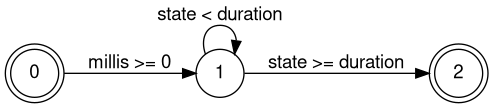
\includegraphics[width=8cm]{fig/wait.png}
    \caption{The Sys.wait function as a diagram.}
    \label{fig:wait-dfa}
  \end{figure}
\end{center}
The first time the function is called, the state is \(0\), so we should enter the second if-statement.
Unless the user passed a zero as the time to be waited, the function returns \(1\) as the next state.
When the emulator executes the next step, it checks its internal call stack, which contains the \verb+Sys.wait+ call with state \(1\) as the top element.
For that reason, instead of executing the next statement, the emulator calls the wait function again, but this time with a state of \(1\).
This means that the function then returns a new state of \(2\).
This loop then continues until the state is the same size as the first argument multiplied by 1000.
When this happens, the original first argument is returned inside the special finished state, which means that the function should be removed from the emulator's internal call stack and the next statement can finally be executed.
The multiplication by 1000 is relatively arbitrary here, since the actual duration depends on the current tick rate, which is a feature of the user interface and therefore unknown to the emulator~\ref{step-by-step}.
It would be theoretically better to first set the status to the current system time and then decrement it until it reaches zero again.
At the moment, however, this is not possible because WebAssembly does not provide an API for accessing the system time.
\begin{lstlisting}[
  language=Rust,
  label={lst:sys.wait},
  caption={Implementation of the Sys.wait function},
  captionpos=b
  ]
  pub fn wait(_vm: &mut VM, state: State, params: &[Word]) -> StdResult {
    if params[0] < 0 {
        return Err(StdlibError::SysWaitNegativeDuration);
    }

    let duration = params[0] as State * 1000;
    if state < duration {
      return Ok(StdlibOk::ContinueInNextStep(state + 1));
    }

    Ok(StdlibOk::Finished(params[0]))
  }
\end{lstlisting}

\subsubsection{Example: Output.printString} \label{complex-example}
% or Keyboard.readLine (also shows why you can't just execute the entire native function)
\cref{lst:output.printstring} shows a more complicated function which uses the system described above.
This function can be used to output an entire string to the emulator's screen.
It does not implement all of the functionality itself, instead relying on the string module to iterate over the characters, and the output module's printChar function to print just a single character.
In theory, this function would be trivial, a simple for loop from zero to the length of the string, with only a single call to the printChar function as the loop body.
Yet it is not trivial in practice due to the limitations described in~\cref{stdlib-issues}.
\begin{center}
  \begin{figure}[ht]
    \centering
    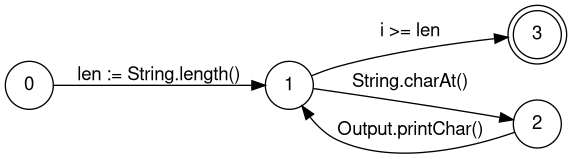
\includegraphics[width=10cm]{fig/printString.png}
    \caption{The Output.printString function as a diagram.}
    \label{fig:printstring-dfa}
  \end{figure}
\end{center}
Each time a function is called within a standard native library function, the latter must be stopped, since the former might be a function written in bytecode, and therefore subject to the user interface's stepwise debugger.
For example, if the native output implementation is used in combination with a string implementation in bytecode, the user might reasonably expect to step through the charAt function called by the printString function in the user interface.
This is indeed possible with this system.
Features like this necessitate the complexity of these native implementations, as they cannot be implemented with a normal for loop.
In the future, it may be possible to implement this in Rust in a more idiomatic way using the planned yield statement, however this is still a proposal at the time of writing.
Most of the logic is explained in the comments of~\cref{lst:output.printstring}, but the basic idea is simply to use the state argument both as an index for the loop and to store the length of the string.
This is possible because the state type is a 32-bit integer, whereas the VM emulator uses only 16-bit integers, so the state can contain two different values.
Depending on whether the state is even or odd, we alternately call the charAt or printChar function until everything has been printed.
Although the function is actually rather simple, it appears quite complicated in the code, so it is shown again in~\cref{fig:printstring-dfa}, but this time in a graphical representation of the state machine.
Each state transition in the graphical representation is a suspension point for the function, with the transition to state \(3\) representing the final return in line 28 of the code.

\begin{lstlisting}[
  language=Rust,
  label={lst:output.printstring},
  caption={Implementation of the Output.printString function},
  captionpos=b
  ]
  pub fn print_string(vm: &mut VM, state: State, params: &[Word])
  -> StdResult {
    // State is 32 bits wide. The upper 16 bits are used to keep
    // the length information, while
    // the lower 16 bits are used for the actual state counter
    let string = params[0];
    let real_state = state & 0xFFFF;

    // in the first tick: get the length of the string to be printed
    if state == 0 {
      return call_vm!(vm, state, "String.length", &[string]);
    }

    // the second call of this function is a special case, because the
    // string length is on the stack instead of in the state
    let (len, last) = if state == 1 {
      (vm.pop()? as State, 0)
    } else {
      ((state >> 16) & 0xFFFF, vm.pop()?)
    };

    // we need 2 ticks for each i, so divide by 2
    // also subtract 1 because this will not be executed for state 0
    let i = (real_state as Word - 1) / 2;

    // the exit condition
    if i >= len {
      return Ok(Finished(0));
    }

    // keep alternating between these 2 while i < len
    if is_odd(state) {
      vm.call("String.charAt", &[string, i])?;
      Ok(ContinueInNextStep((len << 16) | (state + 1)))
    } else {
      vm.call("Output.printChar", &[last])?;
      Ok(ContinueInNextStep((len << 16) | (state + 1)))
    }
  }
\end{lstlisting}

\subsection{Integrating the emulator into the Web UI}
So far, all sections have dealt with the internals of the emulator.
The primary goal of the project, however, is to provide the user with a web-based interface.
Integrating the emulator into a web page is done by first compiling the Rust code into a Wasm library, which is then used by a ReactJS application~\ref{react-js}.
The exact boundary between JavaScript and Rust is arbitrary and has actually changed during the development of the application.
In the finished version, the JavaScript code requests the current frame of the screen from the Rust code, which then renders the pixel data into a JavaScript ImageData buffer, a type provided by the web-sys crate~\ref{web-sys}, and returns it.
The JavaScript code then simply displays the data inside a normal canvas element.
In fact, the Rust code doesn't do anything by itself, it just provides functions that can be used by the ReactJS application.
Another example of this principle is the handling of keyboard events, which are received by JavaScript, then passed to Rust and processed accordingly inside the emulator.
So the main loops, both for running the VM and for displaying the current frame, are written in JavaScript.
To improve performance, however, the step calls to the VM are batched.
When the emulator runs in a loop, a single iteration of the loop in the interface actually corresponds to thousands of ticks for the emulator, depending on the position of the speed slider~\ref{ui-showcase}.
This does not happen during debugging, of course, where a single step in the user interface usually corresponds to a single tick in the emulator.
The only exception to this rule is that the front-end automatically keeps ticking as long as the emulator is executing a built-in standard library function.
The reason for this becomes immediately clear when one looks at~\cref{sys.wait-example}.
It is not desirable to click the step button a thousand times for every second you want the emulator to wait.
By giving the front-end control over all execution, state implementation becomes much simpler, as all user interface elements can be easily updated after an event causes a change in emulator state.
If this were not the case, the emulator would have to notify the front-end of state changes, or the UI would have to actively ask the emulator for its current state as often as possible.
The interaction between the JavaScript front-end and the emulator code is facilitated by a thin compatibility layer in Rust.
This layer provides a unified interface to the front-end that works for both the VM and the CPU emulators.
As a result, there is no need to implement two different user interfaces, and all JavaScript code is shared between the two emulators.

\subsection{Web UI showcase} \label{ui-showcase}
The web-based user interface is shown in~\cref{fig:ui-demo-desktop}.
It is divided into four major parts.
Above everything else, there is a row with all interactive UI elements.
This row contains the buttons for loading a new program, starting, stopping, advancing a single step or resetting the running program and the slider for changing the VM execution speed.
In the middle left part of the image the bytecode of the currently loaded program is displayed.
This information is useful when the user is using the ``Step'' button to debug the loaded program.
The instruction to be executed next is highlighted in red.
To the right of that is the most important part of the user interface, the emulator screen.
Here the screen section of the emulator memory is displayed.
Below those two, certain parts of the internal memory are shown to improve the debugging experience.
From left to right, those are the call stack, local variables, arguments to the current function and the stack.
These fields are updated each time the emulator comes to a stop, i.e.\ after each step or after pressing the stop key.
Since the emulator executes thousands of ticks per second, updating the values after each tick would be neither feasible nor useful, so they are only updated after stopping~\ref{ui-compatibility}.
If they are not updated while running, there is no point in displaying them at all, so the bytecode view and the memory segments are hidden while the program is running.
This allows the screen to fill almost the entire browser window and its contents to become as large as possible.
In contrast, the button row at the top and the screen are always visible.
\begin{center}
  \begin{figure}[ht]
    \centering
    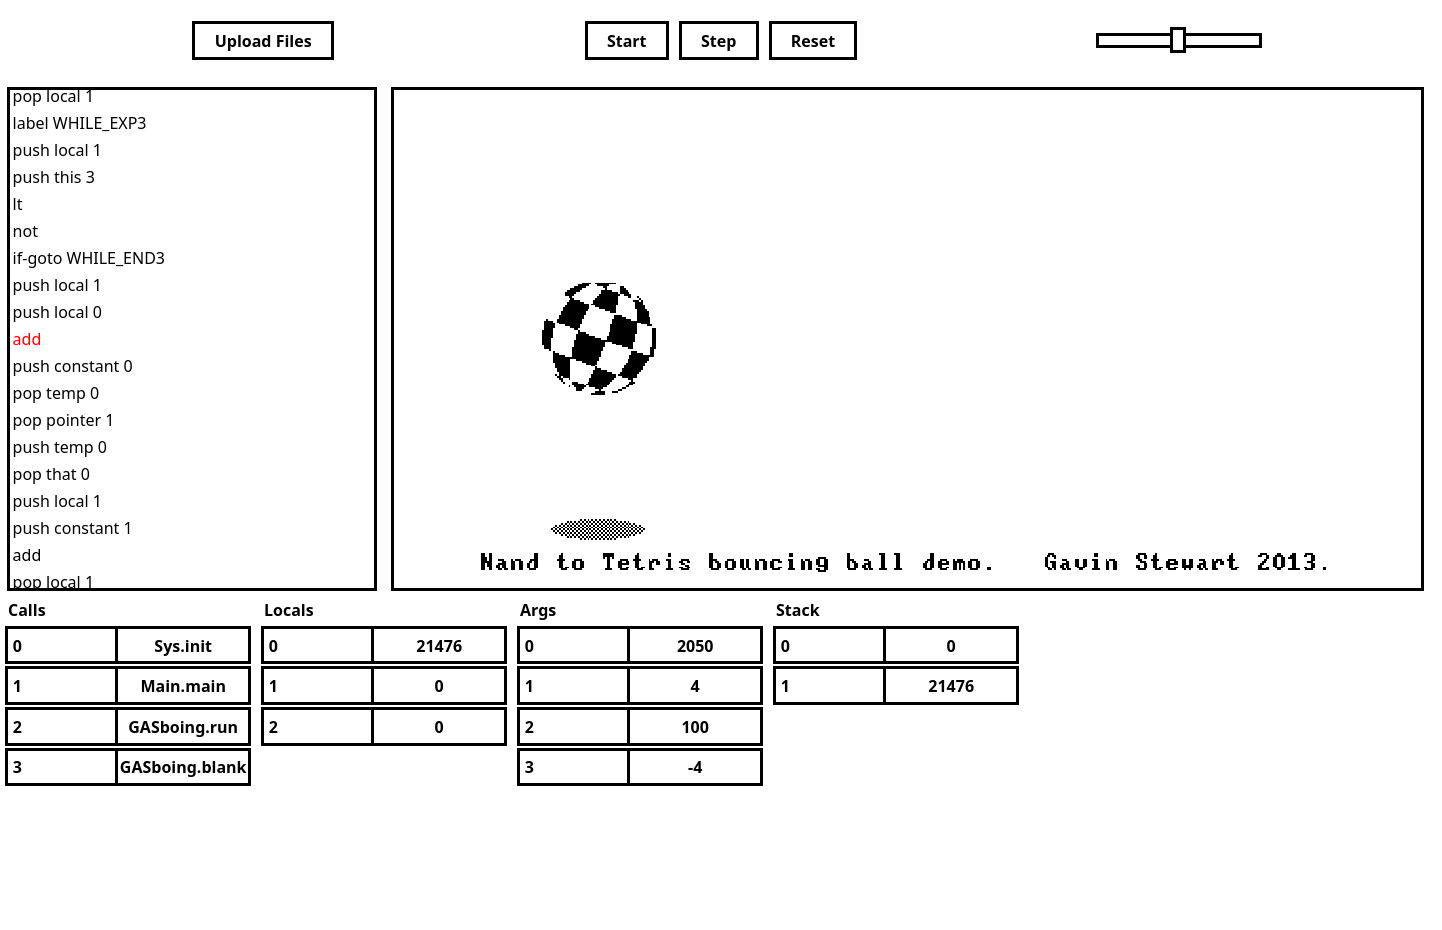
\includegraphics[width=12cm]{fig/ui-demo-desktop.png}
    \caption{The web-based user interface on a desktop computer.}%
    \label{fig:ui-demo-desktop}
  \end{figure}
\end{center}
One of the biggest advantages of web-based applications is the ability to use them without a local installation, simply by opening a link in the user's web browser.
This only works if the application is hosted on a public web server.
For many applications, this means renting or operating an expensive server infrastructure for the backend of their service.
In contrast, the new emulators are compiled to WebAssembly, which allows them to run entirely in the client's web browser.
This means that no backend is needed and therefore a simple static file server is sufficient to host the entire application.
GitHub offers such a file hosting service free of charge.
It is called ``GitHub Pages'' and allows users to host static web resources by simply uploading them to a directory on GitHub's servers and marking that directory as public in the repository settings.
In addition, GitHub offers a service called ``GitHub Actions'' that allows arbitrary code to be executed on Microsoft's servers depending on various events in the repository, such as a push to the main branch.
Combining these two services, one can automatically build and deploy the entire WebAssembly application to Pages every time there is a push to the main branch.
That is exactly what this project does, even though it is technically hosted on the HHU's internal GitLab instance.
Every time there is a push to the GitLab instance, that push is automatically mirrored to GitHub, which then builds the Wasm and JavaScript code and deploys it to GitHub Pages.
